\documentclass[10pt]{exam}
\firstpageheader{Math 2550 Fall 2020}{Homework 4}{Instructor:  J. Haga}
\usepackage{amsfonts}
\usepackage{amsmath}
\usepackage{amssymb, graphicx, enumerate, mathrsfs}
\begin{document}


\newcommand{\dd}{\textrm{d}}
\newcommand{\NN}{\mathbb N}
\newcommand{\CC}{\mathbb C}
\newcommand{\QQ}{\mathbb Q}
\newcommand{\ZZ}{\mathbb Z}
\newcommand{\RR}{\mathbb R}
\newcommand{\proofdone}{\hfill $\square$}

\noindent Due:  Monday, October 19  \\
\vskip 0.5cm
\begin{questions}
\question 
\begin{parts}
\part Provide two predicates $P(x)$ and $Q(x)$ (and a domain $D$ for the variable $x$) for which $$[\forall x\in D \,\,(P(x)\vee Q(x))]\,\, \Rightarrow\,\, [(\forall x \in D,\, P(x)) \vee (\forall x \in D,\, Q(x))]$$ is false.
\\\emph{Solution.}\\
$P(x) = x$ is even, $Q(x) = x$ is odd, $D = \NN$
\vfill
\part Provide a predicate $P(x,y)$ (and domains $D_x$ and $D_y$ for the variables $x$ and $y$ respectively) for which $$[\forall y\in D_y,\,\, \exists x\in D_x\,\,\textrm{s.t.}\,\, P(x,y)]\,\,\Rightarrow \,\,[\exists x\in D_x\,\,\textrm{s.t.}\,\, \forall y\in D_y\,\, P(x,y)]$$ is false.
\\\emph{Solution.}\\
$D_y = \RR, D_x = \RR, P(x, y): y/x = 1$ 
\vfill
\end{parts}

\newpage

\question Suppose that $A$, $B$, $C$, and $D$ are sets for which
\begin{itemize} 
\item $A\cup B \subseteq C\cup D$, 
\item $A\cap B = \varnothing$, and 
\item $C\subseteq A$.  
\end{itemize}
Prove that $B\subseteq D$.\\
%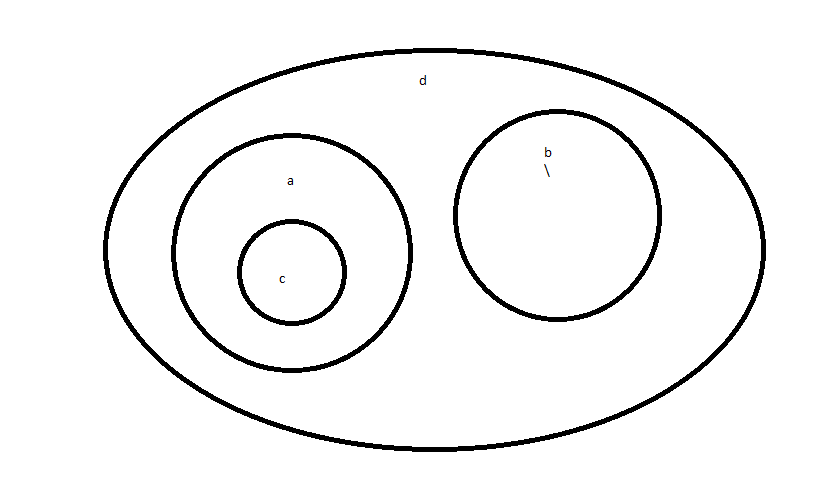
\includegraphics[scale = .7]{number2.png}\\
\emph{Solution.}\\
Assume $A\cup B \subseteq C\cup D$, $A\cap B = \varnothing$, and $C\subseteq A$. Let $x \in A\cup B$. 
Then, since $x \in A\cup B$ and $A\cup B \subseteq C\cup D$, $x \in C\cup D$. Since $A\cap B = \varnothing$, 
$x$ must be in $A$ or $B$. Let $x \in B$. Then, since $B \subseteq C\cup D$, $B\subseteq C$ or $B\subseteq D$. 
Let $B \subseteq C$. Then, $x \in B \subseteq C$. Since $C \subseteq A$, $x \in B \subseteq C \subseteq A$
therefore, $x \in A$. Thus we have found that if $x\in B$ and $B \subseteq C$, $x$ must also be in A. 
Since $x \in A\cap B$, $A\cap B \neq \varnothing$, which results in a contradiction since we assumed
that $A\cap B = \varnothing$. Thus, it must be the case that $B \subseteq D$. 

\newpage

\question 
\begin{parts} \part Prove or disprove: for any sets $A$ and $B$, that $$\mathscr P(A\cap B) = \mathscr P(A)\cap \mathscr P(B).$$
Case $\mathscr P(A\cap B) \subseteq \mathscr P(A) \cap \mathscr P(B)$: \\
Let $X \in \mathscr P(A\cap B)$. Then, since $X \in \mathscr P(A\cap B), X\subseteq A\cap B$. 
Since $X \subseteq A\cap B, X\subseteq A$ and $X\subseteq B$. Since $X\subseteq A$, 
$X\in \mathscr P(A)$. Since $X\subseteq B$, $X\in \mathscr P(B)$. Then, since $X$ is in 
both $\mathscr P(A)$ and $\mathscr P(B)$, $X$ is in $\mathscr P(A\cap B)$. Since $X$ was 
arbitrary, $\mathscr P(A\cap B) \subseteq \mathscr P(A) \cap \mathscr P(B)$. \\

Case $\mathscr P(A) \cap \mathscr P(B) \subseteq \mathscr P(A\cap B)$: \\
Let $X \in \mathscr P(A) \cap \mathscr P(B)$. Then, $X\in \mathscr P(A)$ and $X\in \mathscr P(B)$. 
Since $X\in \mathscr P(A)$, $X \subseteq A$. Since $X\in \mathscr P(B)$, $X \subseteq B$
Since $X \subseteq A$ and $X\subseteq B$, $X\subseteq A\cap B$. Since $X\subseteq A\cap B$, 
$X\in \mathscr P(A\cap B)$. \\

Thus, we have shown that both are subsets of the other, therefore are equal. \\

\part Prove or disprove: for any sets $A$ and $B$, that $$\mathscr P(A\cup B) = \mathscr P(A)\cup \mathscr P(B).$$
Counter example: Let $A = \{a, b\}$ and $B = \{b, c\}$. Then, $A\cup B = \{a, b, c\}$ and 
$\mathscr P(A\cup B) = \{\{\},\{a\},\{b\},\{c\},\{a,b\},\{a, c\},\{b, c\},\{a,b, c\}\}$.
However, $\mathscr P(A) \cup \mathscr P(B) = \{\{\}, \{a\}, \{b\}, \{c\}, \{a, b\}, \{b, c\}\}$
Therefore, while $\mathscr P(A) \cup \mathscr P(B) \subseteq \mathscr P(A\cup B)$, 
$\mathscr P(A\cup B) \subsetneq \mathscr P(A) \cup \mathscr P(B)$, and therefore, 
$\mathscr P(A\cup B) \neq \mathscr P(A)\cup \mathscr P(B)$. \\

\part Prove or refute the existence of suitable conditions on sets $A$ and $B$ that guarantee $$\mathscr P(A)\cap \mathscr P(B)=\varnothing.$$
\\
Assume $A$ and $B$ are disjoint. Then, $A\cap B = \varnothing$. Then, $\mathscr P(A\cap B)
= \mathscr P(\varnothing)$. By a previously proven theorem, $\mathscr P(A\cap B) = \mathscr P(A)\cap \mathscr P(B)$. 
Therefore, $\mathscr P(A\cap B) = \mathscr P(A)\cap \mathscr P(B) = \mathscr P(\varnothing) = \varnothing$. 
Thus if $A$ and $B$ are disjoint sets, the intersection of their power sets is the null set. 
\vfill
\end{parts}
\newpage
\question 
\begin{parts}
\part Find the intersection and union of the following family:$$\displaystyle{\mathscr F =\left \{\left[\frac{1-n}{n},\frac{n-1}{n}\right]\,\,:\,\,n\in \NN \right\}}$$
$\bigcup\limits_{F \in \mathscr F} = \{(-1, 1)\}$  \vskip3em
$\bigcap\limits_{F \in \mathscr F} = \{0\}$ 
\newpage
\part Find the intersection and union of the following family:$$\mathscr M = \{n\ZZ:n\in \NN\},$$ where $n\ZZ = \{\dots,-3n,-2n,-n,0,n,2n,3n,\dots\}$ for each $n\in \NN$.
\vskip3em
$\bigcup\limits_{M \in \mathscr M} = \ZZ$  \vskip3em
$\bigcap\limits_{M \in \mathscr M} = 0$ 
\newpage
\part Find the intersection and union of the following family:$$\mathscr V = \{V_n\,\,:\,\,n\in \NN\}$$ where for each natural number $n$, $$ V_n = \{(x,y)\in \RR^2 \,\,:\,\,0\leq x\leq 1,\,x^n\leq y\leq \sqrt[n]x\}.$$
$\bigcup\limits_{V \in \mathscr V} = \{(x,y)\in \RR^2 \,\,:\,\,0\leq x\leq 1,\,0\leq y\leq 1\}$  \vskip3em
$\bigcap\limits_{V \in \mathscr V} = \{(x, y)\in \RR^2 \,\,:\,\, x = y, 0\leq x\leq 1,\,0\leq y\leq 1\}$ 
\newpage
\end{parts}



\end{questions}


\end{document}